\documentclass[useAMS, usenatbib]{mnras}
\pdfsuppresswarningpagegroup=1
%
\usepackage[spanish,es-minimal,english]{babel}
\usepackage[utf8]{inputenc}
\usepackage{graphicx}

\usepackage{xcolor}
\usepackage{hyperref}
\usepackage{siunitx}
\usepackage{newtxtext}
\usepackage[stix2,smallerops]{newtxmath}
\usepackage{booktabs}
\hypersetup{colorlinks=True, linkcolor=blue!50!black, citecolor=black,
  urlcolor=blue!50!black}
\usepackage{etoolbox}
\robustify\bfseries
\robustify\itshape

\usepackage[shortlabels]{enumitem}

\bibliographystyle{mnras}

\sisetup{
  % explicit "+" is useful for velocities
  retain-explicit-plus = true,
  % prefer 10^6 over 1 x 10^6
  retain-unity-mantissa = false,
  % Use x +/- e instead of x(e)  
  separate-uncertainty = true,
  % Make sure to pick up bold font when used in section heading for instance
  detect-weight = true,
}

%% 
%% Will macros
%%
% A better \ion command that works in more circumstances
\newcommand\ION[2]{#1\,\scalebox{0.9}[0.8]{\uppercase{#2}}}
\newcounter{ionstage}
\renewcommand{\ion}[2]{\setcounter{ionstage}{#2}% 
  \ensuremath{\mathrm{#1\,\scriptstyle\Roman{ionstage}}}}
\newcommand\hii{\ion{H}{2}}
\newcommand\nii{[\ion{N}{2}]}
\newcommand\oiii{[\ion{O}{3}]}
\newcommand\oii{[\ion{O}{2}]}
\newcommand\Wav[1]{\ensuremath{\lambda #1}}

\title[HH 529 II and III in the Orion Nebula]{
  Photoionized Herbig-Haro objects in the Orion Nebula I: HH 529 II and III
}

\author[J. E. M\'endez-Delgado et al.]
{J. E. M\'endez-Delgado$^{1,2}$ \thanks{E-mail: jemd@iac.es},
  C. Esteban$^{1,2}$, J. Garc{\'{\i}}a-Rojas$^{1,2}$, W. J. Henney$^{3}$  
  \newauthor 
  and K. Z. Arellano-C\'ordova$^{1}$ and collaborators\\
\\
% List of institutions
$^{1}$Instituto de Astrof\'isica de Canarias (IAC), E-38205 La Laguna, Spain\\
$^{2}$Departamento de Astrof\'isica, Universidad de La Laguna, E-38206 La Laguna, Spain\\
$^{3}$Instituto de Radioastronom\'ia y Astrof\'isica, Universidad Nacional Aut\'onoma de M\'exico, Apartado Postal 3-72, 58090 Morelia, Michoac\'an, M\'exico}


\begin{document}

\begin{table}
  % Fake the labels for some Tables
  \setcounter{table}{3}\caption{}\label{tab:pc}
  \setcounter{table}{12}\caption{}\label{tab:total_abundances_rls}
\end{table}

\addtocounter{section}{11}
\section{Physical aspects of the high velocity components}
\label{sec:phys-aspects-high}


\newcommand\Mach{\ensuremath{\mathcal{M}}}
\newcommand\shock{\ensuremath{_{\mathrm{sh}}}}
\newcommand\sound{\ensuremath{c_{\mathrm{s}}}}
\newcommand\ws{\ensuremath{_{\mathrm{ws}}}}
\newcommand\jet{\ensuremath{_{\mathrm{jet}}}}
\newcommand\env{\ensuremath{_{\mathrm{env}}}}
Since the material in the HH outflows is moving highly supersonically
with respect to the ionized sound speed in the nebula,
it will give rise to shocks where the flow and nebula interact
\citep{Hartigan:1987a}.
Further internal shocks may form inside the outflow
if its velocity varies with time \citep{Raga:1990a}.
It is important to investigate the degree to which direct excitation by the shocks
might be affecting our emission line analysis.

In this section,
we first calculate the heating and compression expected behind a shock wave.
Second, we estimate the range of likely shock velocities expected to be
found in the HH~529 knots.
Third, we use results of non-equilibrium Cloudy simulations to predict the relative contributions of the post-shock cooling zone and the
equilibrium photoionized shell to the emission line spectrum of the knots.

\subsection{Shock compression and heating}
\label{sec:shock-compr-heat}

A non-magnetised hydrodynamic shock is characterized by its Mach number \(\Mach = V\shock / \sound\),
where \(V\shock\) is the shock velocity and \(\sound\) is the pre-shock adiabatic sound speed.
On passing through the shock, the gas is heated 
\citep{ZelDovich:1967a} to a temperature \(T_1\),
which is higher than the equilibrium photoionized temperature, \(T_0\):
\begin{equation}
  \label{eq:T1-T0}
  \frac{T_1}{T_0} = \frac{1}{16} \bigl( 5 \Mach^2 - 1 \bigr)
  \bigl( 1 + 3\Mach^{-2} \bigr),
\end{equation}
while at the same time it is compressed by a factor
\begin{equation}
  \label{eq:rho1-rho0}
  \frac{\rho_1}{\rho_0} = \frac{4 \Mach^2}{\Mach^2 + 3} .
\end{equation}
In both cases, a ratio of specific heats \(\gamma = 5/3\) is assumed,
as is appropriate for ionized and atomic gas. 
The post-shock gas then cools in a radiative relaxation layer
until it returns to the equilibrium temperature \(T_2 \approx T_0\),
reaching a final density compression factor of 
\begin{equation}
  \label{eq:rho2-rho0}
  \frac{\rho_2}{\rho_0} = \frac53 \Mach^2 .
\end{equation}

The adiabatic sound speed in the equilibrium ionized gas is given by
\(\sound = (\gamma k T / \mu m_{\mathrm{H}})^{1/2}\),
where \(k\) is the Boltzmann constant, \(T\) is the temperature,
\(m_{\mathrm{H}}\) is the hydrogen mass
and \(\mu\) is the mean atomic mass per particle.
Assuming that all He is singly ionized with
\(y = \mathrm{He/H} = 0.087\) (Table~\ref{tab:total_abundances_rls}) yields
\(\mu \approx (1 + 4 y) / (2 + 2 y) \approx 0.62\),
which combined with \(T = \SI{8480}{K}\) (Table~\ref{tab:pc})
implies an adiabatic sound speed of \(\approx\SI{13.7}{km.s^{-1}}\). 

The case of a magnetized shock is considerably more complicated \citep{Bazer:1959a},
but the principle effect is that the component of the magnetic field, \(B\), parallel to the shock front provides extra pressure support (magnetic cushioning) in the post-shock gas \citep{Hartigan:1994a}.
An approximate way to account for this is to replace the sound speed in the above equations by the fast magnetosonic speed: \(V_{\text{fast}} = (\sound^2 + V_{\text{A}}^2)^{1/2}\), where \(V_{\text{A}} = B / (4\pi \rho)^{1/2}\)
is the Alfvén speed.
The ambient gas inside an \hii{} region is expected to have a low
Alfvén speed of \(V_{\text{A}} \approx \SI{2}{km.s^{-1}} \ll \sound\)
\citep{Arthur:2011a}
so that the magnetic cushioning will be negligible
in shocks propagating in the ambient medium.
On the other hand,
the Alfvén speed in the jet itself \citep{Hansen:2015b, Pudritz:2019a}
may be sufficiently high so as to limit the compression behind
shocks driven into the jet.

\subsection{Shock velocities in jet working surfaces}
\label{sec:shock-velocities-jet}


\begin{figure}
  \centering
  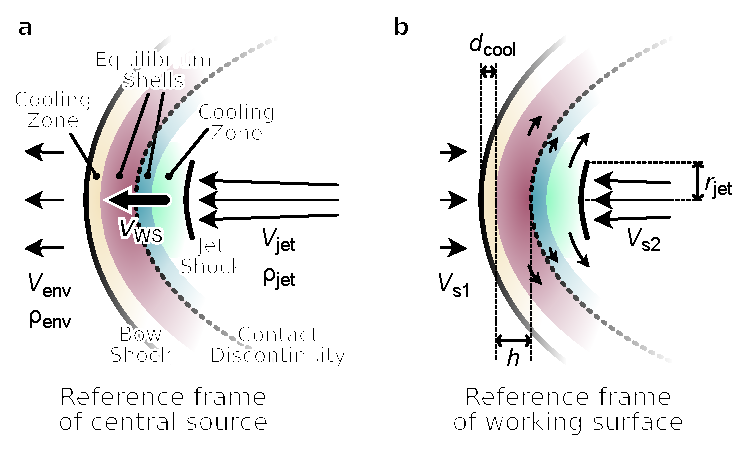
\includegraphics[width=\linewidth]{working-surface-diagram}
  \caption{
    Structure of a fully photoionized jet knot,
    modeled as a steady-state working surface,
    which forms when a jet propagates supersonically into an environment.
    (a)~Velocities in the frame of reference of the central jet source.
    (b)~Velocities in the frame of reference of the working surface.
  }
  \label{fig:working-surface}
\end{figure}

\begin{figure}
  \centering
  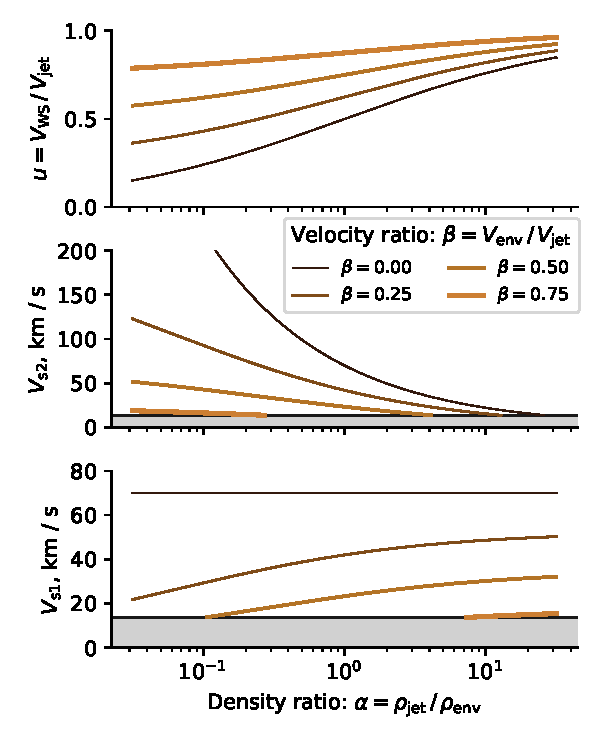
\includegraphics[width=\linewidth]{shock-velocities}
  \caption{Inner and outer shock velocities of a working surface
    as a function of the jet-to-environment ratio of density and velocity
    (\(\alpha\) and \(\beta\)).
    Colored dots show plausible parameters for the working surface in
    HH~529~II (red dots) and
    HH~529~III (light and dark blue dots).
    Upper panel shows the pattern speed of the working surface, \(V\ws\),
    in terms of the jet velocity, \(V\jet\).
    Middle panel shows the velocity of the jet shock, \(V_{\mathrm{s1}}\),
    for the case where \(V\ws = \SI{65}{km.s^{-1}}\).
    The gray shaded area indicates subsonic velocities where no shock exists. 
    Bottom panel is the same but for the bow shock \(V_{\mathrm{s2}}\).
  }
  
  \label{fig:shock-velocities}
\end{figure}

Figure~\ref{fig:working-surface} illustrates a simplistic model of the structure of a jet knot.  An outer shock (the bow shock) accelerates the environment, while an inner shock (the jet shock or Mach disk) decelerates the jet.
The region between these two shocks comprises shocked environment and jet material in approximate pressure equilibrium,
which is denoted the working surface.\footnote{
  In reality, the knot structure may be more complicated
  with internal clumps \citep{Hansen:2017a, Yirak:2009a, Yirak:2012a}
  and the possibility of double working surfaces \citep{Raga:2017b}.  
}
The speed of the working surface with respect to the jet source, \(V\ws\),
will only be a fraction of the jet speed: \(u \equiv V\ws / V\jet\)
(see Figure~\ref{fig:working-surface}a),
depending on the velocities and densities of the jet and environment,
which we characterize by the ratios \(\alpha = \rho\jet/\rho\env\) and \(\beta = V\env/V\jet\).
For the terminal working surface with which the jet interacts directly with the nebula, one expects \(\beta \approx 0\),
whereas internal working surfaces due to jet variability may have \(\beta \sim 0.5\).

Assuming that the momentum transfer efficiency
to the working surface from the jet
is the same as that from the environment,
then pressure balance along the jet axis
in the frame of the working surface can be written:
\newcommand\subs[1]{\ensuremath{_{\text{s#1}}}}
\begin{equation}
  \label{eq:pressure-balance}
  \rho\env \bigl( V\subs1^2 + \sound^2/\gamma \bigr)
  = \rho\jet \bigl( V\subs2^2 + \sound^2/\gamma \bigr)
  = \rho\ws \sound^2/\gamma ,
\end{equation}
where \(V\subs1 = V\ws - V\env\) and \(V\subs2 = V\jet - V\ws\)
are the respective speeds with which material enters the bow shock
and the jet shock (see Figure~\ref{fig:working-surface}b).
For simplicity of exposition, this ignores both the magnetic field
and the weak density dependence of the photoionized equilibrium temperature. 
Substituting the definitions of \(u\), \(\alpha\), \(\beta\),
and solving for \(u\) yields
\begin{equation}
  \label{eq:u}
  u = \frac{
    \bigl[
    \alpha (1 - \beta)^2 - (1 - \alpha) \bigl( \beta^2 - \alpha \bigr) \Mach\ws^{-2}
    \bigr]^{1/2} - (\alpha - \beta)
  }{
    (1 - \alpha) \bigl( 1 + \Mach\ws^{-2} \bigr)
  } , 
\end{equation}
where \(\Mach\ws = \gamma^{1/2} V\ws/\sound\) is the \emph{isothermal} Mach number corresponding to the working surface velocity. 
The shock velocities are then given in terms of the working surface velocity as  
\(V\subs1 = (u - \beta) V\ws /u \) for the bow shock,
and \(V\subs2 = (1 - u) V\ws /u \) for the Mach disk.

The quantities \(u\), \(V\subs1\), and \(V\subs2\) are plotted in Figure~\ref{fig:shock-velocities} as a function of the density ratio \(\alpha\)
for four different values of the ambient velocity \(\beta\).
A working surface velocity of \(V\ws = \SI{65}{km.s^{-1}}\)
(\(\Mach\ws \approx 6.1\)) is assumed,
which is a typical average value for the HH~529 knots observed in this paper.
For an over-dense jet (\(\alpha > 1\)), the ratio \(u\) tends to unity,
meaning that the working surface moves with the jet velocity.\footnote{
  Note that there is a maximum density ratio of \(\alpha = 1 + (1 - \beta)^2 \Mach\ws^2\),
  beyond which there is no steady state solution for a fully ionized working surface.
  For jets that are denser than this, the thermal pressure of the jet exceeds any possible confining ram pressure.
}
For an under-dense jet (\(\alpha < 1\)), the ratio \(u\) becomes smaller,
meaning that the jet velocity significantly exceeds that of the working surface.
This effect is particularly marked for the case of a static environment (\(\beta = 0\)), where it would predict a jet shock velocity, \(V\subs2\), of hundreds of \si{km.s^{-1}}.  On the other hand, the bow shock velocity,
\(V\subs1\), is always equal to \(V\ws\) for \(\beta = 0\), whatever the value of \(\alpha\).

What values of \(\alpha\) and \(\beta\) are appropriate for the HH~529 knots?
For an internal working surface, which probably applies to HH~529~II,
both the ``jet'' and ``environment''
are really just different sections of the same jet that were ejected at different times.
The value of \(\beta\) is therefore related to the relative amplitude
\(\Delta V/V_0\) of temporal variations in the jet velocity
as \(\beta > (1 - \Delta V/V_0) / (1 + \Delta V /V_0)\).
Studies of other HH jets \citep{Raga:1998a, Esquivel:2007a, Castellanos-Ramirez:2018a} suggest \(\Delta V/V\jet \le 0.3\), implying \(\beta \ge 0.5\).  On the other hand, a value as high as \(\beta = 0.75\) (thick yellow lines in Figure~\ref{fig:shock-velocities}) would give subsonic values of \(V\subs1\) and \(V\subs2\) for all but a narrow range of \(\alpha\), which is inconsistent with the model of a shock-bounded working surface,
so a value of \(\beta \approx 0.5\) is more reasonable.
If the jet mass-loss rate is roughly constant
over the period of the velocity variation, then mass continuity implies
\(\rho\jet V\jet \approx \rho\env V\env\), which yields \(\alpha \approx \beta\).
If we assume \(\alpha = \beta = 0.5 \), then from equation~\eqref{eq:u} we find
\(u = 0.70 \), from which the jet velocity follows as
\(V\jet = V\ws / u \approx \SI{93}{km.s^{-1}}\)
and the shock velocities as
\(V\subs1 = \SI{19}{km.s^{-1}}\) for the bow shock and
\(V\subs2 = \SI{28}{km.s^{-1}}\) for the jet shock.
This solution is indicated by red dots in Figure~\ref{fig:shock-velocities}.
Given that the derived electron density in the HH~529~II working surface is
\(n\ws \approx \SI{12000}{cm^{-3}}\) (Table~4),
and assuming no significant changes in ionization,
one finds \(n\env = n\ws / 4.0 \approx \SI{3000}{cm^{-3}}\)
and \(n\jet = n\ws / 8.0 \approx \SI{1500}{cm^{-3}}\).



Although it is conceivable that HH~529~III is also an internal working surface, its large-scale bow shock appearance suggests that it may instead be a terminal working surface that interacts directly with the ambient nebula.  The internal velocity dispersion within the nebula \citetext{\(\approx \SI{6}{km.s^{-1}}\), \citealp{Arthur:2016a}}
is much smaller than \(V\jet\), so we will assume \(\beta = 0\).
If we further suppose that the jet velocity feeding this working surface is the same \(V\jet \approx \SI{93}{km.s^{-1}}\)
as in HH~529~II, then it follows that \(u = 0.74\) and \(\alpha \simeq 7\).
This then implies shock velocities of \(V\subs1 = \SI{70}{km.s^{-1}}\)
and \(V\subs2 = \SI{25}{km.s^{-1}}\),
which can be combined with the electron density of the HH~529~III working surface, 
\(n\ws \approx \SI{30000}{cm^{-3}}\) (Table~4),
to find \(n\env = n\ws / 45 \approx \SI{670}{cm^{-3}}\)
and \(n\jet = n\ws / 6.5 \approx \SI{4600}{cm^{-3}}\).
This is a 3 times higher jet density than derived above for HH~528~II,
which is inconsistent with the assumption of a constant mass-loss rate.
We therefore consider the alternative hypothesis that \(\rho\jet V\jet\)
is equal between the two working surfaces,\footnote{
  This is expected for constant mass-loss since the separation
  between II and III
  is much less than the distance from the jet source. 
}
but that \(V\jet\) need not be.
This is approximately satisfied for \(\alpha = 1.5\), which implies \(u = 0.55\)
\(V\jet = \SI{127}{km.s^{-1}}\), \(V\subs2 = \SI{57}{km.s^{-1}}\), \(n\jet = \SI{1000}{cm^{-3}}\) (\(V\subs1\) and \(n\env\) are unchanged from the previous solution).
The two solutions are indicated by light and dark blue dots in Figure~\ref{fig:shock-velocities}. 

\begin{figure}
  \centering
  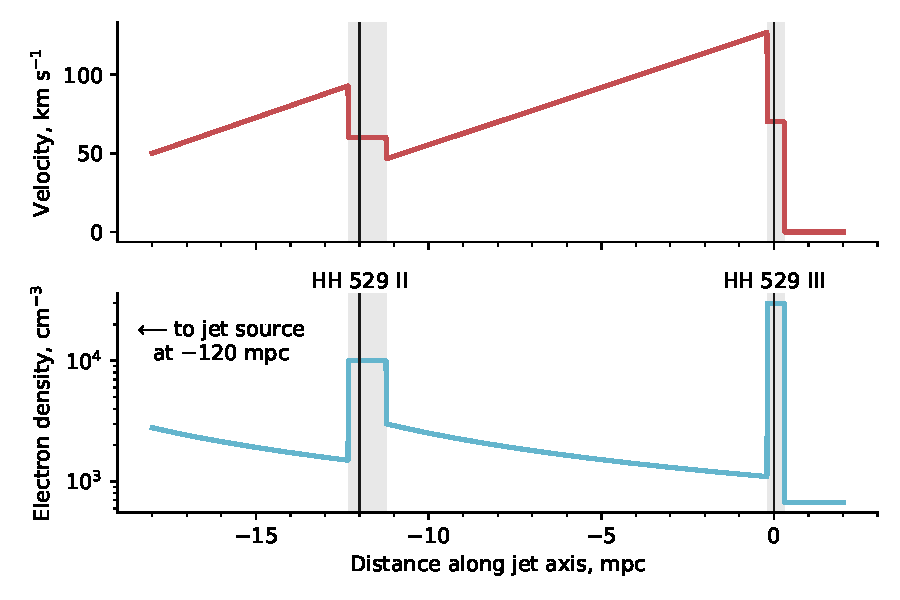
\includegraphics[width=\linewidth]{hh529-ii-iii-ws-profiles}
  \caption{
    Plausible reconstruction of the flow velocity (upper)
    and density (lower)
    for the section of jet covered by the UVES slit.
    The two working surfaces are marked with gray shading,
    with the contact discontinuities indicated by thin vertical lines.
    HH~529~II is an internal working surface, bounded by low-velocity shocks (\num{20} to \SI{30}{km.s^{-1}}),
    while HH~529~III is a terminal working surface, bounded by higher velocity shocks (\num{50} to \SI{70}{km.s^{-1}}).
    Distances along the jet axis are measured in mpc (\(1'' \approx \SI{2}{mpc}\))
    with respect to HH~529~III.
  }
  \label{fig:ws-profiles}
\end{figure}


\citet{Bally:2006a} estimate the mass loss rate of a large sample of photoionized jets in the Orion Nebula, finding that the majority lie in the range \num{e-7} to \SI{e-6}{M_\odot.yr^{-1}}.  



\subsection{Shock emission versus shell emission}
\label{sec:shock-emiss-vers}



\bibliography{will-529-shock-refs}

\end{document}

%%% Local Variables:
%%% mode: latex
%%% TeX-master: t
%%% End:
